\documentclass[12pt]{article}
\usepackage{graphicx}
\usepackage{multirow}
\usepackage{minted}
\usepackage{hyperref}

\title{High-performance Computing, Autumn 2024}
\author{Robert Buj}
\date{\today}

\begin{document}
\maketitle

\section*{Question 1}

Steps:
\begin{enumerate}
	\item compile the source code
\begin{minted}{shell}
make
\end{minted}
	\item queue the jobs using the bash script s2.sh
\begin{minted}{shell}
for p in app app2; do ./s2.sh -n $p; done | sh
\end{minted}
	\item get gnuplot data
\begin{minted}{shell}
for p in app app2; do python3 s4.py -n $p > $p.dat; done
\end{minted}
	\item get gnuplot figure
\begin{minted}{shell}
gnuplot executiontime.gnu
\end{minted}
\end{enumerate}

\begin{figure}[h!]
	\begin{minted}{shell}
qsub -N app_10_1 -v name=app -v size=10 template.sge
qsub -N app_10_2 -v name=app -v size=10 template.sge
...
qsub -N app_1500_10 -v name=app -v size=1500 template.sge
qsub -hold_jid "app_*" -N app_end -v name=app -cwd ./s3.sge
	\end{minted}
	\caption{./s2.sh -n app}\label{code:helper}
\end{figure}


\newpage

\begin{figure}[h!]
	\inputminted{shell}{s2.sh}
	\caption{file s2.sh}\label{code:s2queue}
\end{figure}

\begin{figure}[h!]
	\inputminted{shell}{template.sge}
	\caption{file template.sge}\label{code:template}
\end{figure}

The scheduler will launch the job s3.sge after running all jobs. The script s3.sge reads the output files from ten executions and it generates a csv file for each application argument. The csv file has the following fields:
\begin{itemize}
	\item host name that received and ran the job
	\item execution start of the job (UNIX timestamp)
	\item execution time of the job (seconds)
\end{itemize}

\begin{figure}[h!]
	\inputminted{shell}{s3.sge}
	\caption{file s3.sge}\label{code:endscript}
\end{figure}

\newpage

The following script gets the gnuplot data from the csv obtained in the previous steep, and it calculates the mean execution time and its standard deviation for a certain argument (10, 50, 100, 1000, 1500). 

\begin{figure}[h!]
\inputminted{python}{s4.py}
\caption{file s4.py}\label{code:python3}
\end{figure}

REF: \href{https://www.geeksforgeeks.org/use-pandas-to-calculate-stats-from-an-imported-csv-file/}{Use Pandas to Calculate Stats from an Imported CSV file}

\newpage

\section*{Question 2}

The results are summarized in Figure~\ref{fig:exectime}. The plot below displays the execution time with -O3 optimization and without. The optimized binary got better results.

\begin{figure}[h!]
	\centering
	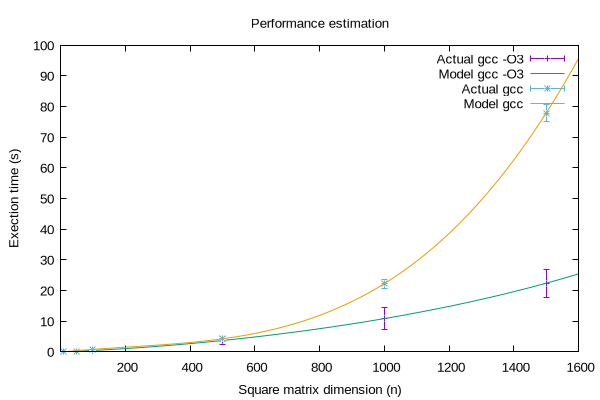
\includegraphics[width=0.9\linewidth]{q2.png}
	\caption{Time needed to run the jobs.}
	\label{fig:exectime}
\end{figure}

Table~\ref{tab:results} summarize the results obtained. At the beginning the execution time grows linearly and later exponentially.

\begin{table}[h!]
	\centering
    \begin{tabular}{|l|r|r|r|r|} 
		\hline
		Parameter & Avg(s) & Std. deviation(s) & Avg(s) -O3 & Std. deviation(s) -O3 \\ [0.5ex] 
		\hline
		10 & 0.040 & 0.031 & 0.055 & 0.028 \\
		50 & 0.253 & 0.158 & 0.157 & 0.175 \\
		100 & 0.860 & 0.097 & 0.473 & 0.258 \\
		500 & 4.243 & 0.854 & 3.692 & 1.320 \\
		1000 & 22.225 & 1.485 & 10.839 & 3.606 \\
		1500 & 77.853 & 2.800 & 22.375 & 4.534 \\
		\hline
	\end{tabular}
	\caption{Summary of results.}
	\label{tab:results}
\end{table}

\newpage

Loop reordering (L.O.) improves execution time over all executions. The loop reordering binary got better results for large matrices: $ N \geq 500 $ with -O3 optimization flag and $ N \geq 100 $ without -O3 optimization flag. The results obtained using the -O3 optimization are summarized in Figure~\ref{fig:exectimeb}.

\begin{figure}[h!]
	\centering
	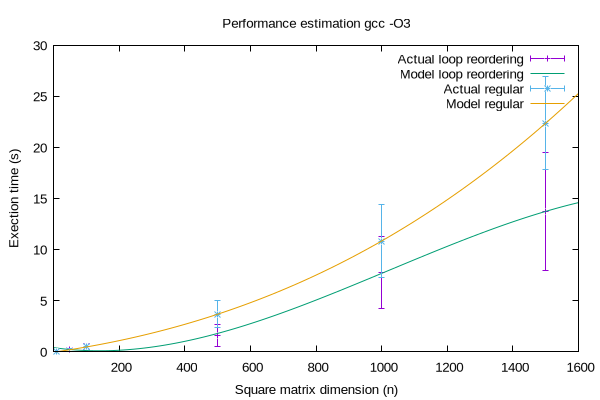
\includegraphics[width=0.9\linewidth]{q2-loop.png}
	\caption{Execution time loop reordering vs regular (gcc -O3).}
	\label{fig:exectimeb}
\end{figure}

\begin{table}[h!]
	\centering
	\begin{tabular}{|l|r|r|r|r|} 
		\hline
		Parameter & Avg(s) & Std. deviation(s) & L.O. Avg(s) & L.O. Std. deviation(s) \\ [0.5ex] 
		\hline
		10 & 0.055 & 0.028 & 0.059 & 0.032 \\
		50 & 0.157 & 0.175 & 0.255 & 0.176 \\
		100 & 0.473 & 0.258 & 0.530 & 0.310 \\
		500 & 3.692 & 1.320 & 1.605 & 1.064 \\
		1000 & 10.839 & 3.606 & 7.761 & 3.481 \\
		1500 & 22.375 & 4.534 & 13.723 & 5.794 \\
		\hline
	\end{tabular}
	\caption{Summary of results for loop reordering vs regular (gcc -O3).}
	\label{tab:resultsb}
\end{table}

\newpage

\begin{figure}[h!]
	\centering
	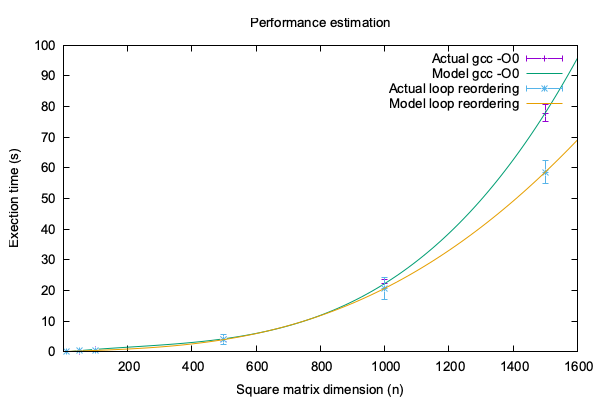
\includegraphics[width=0.9\linewidth]{q2-loopO0.png}
	\caption{Execution time loop reordering vs regular.}
	\label{fig:exectimec}
\end{figure}


\begin{table}[h!]
	\centering
	\begin{tabular}{|l|r|r|r|r|} 
		\hline
		Parameter & Avg(s) & Std. deviation(s) & L.O. Avg(s) & L.O. Std. deviation(s) \\ [0.5ex] 
		\hline
		10 & 0.040 & 0.031 & 0.065 & 0.029 \\
		50 & 0.253 & 0.158 & 0.363 & 0.145 \\
		100 & 0.860 & 0.097 & 0.395 & 0.286 \\
		500 & 4.243 & 0.854 & 3.991 & 1.578 \\
		1000 & 22.225 & 1.485 & 20.678 & 3.661 \\
		1500 & 77.853 & 2.800 & 58.600 & 3.798 \\
		\hline
	\end{tabular}
	\caption{Summary of results for loop reordering vs regular}
	\label{tab:resultsc}
\end{table}

\newpage

\begin{figure}[h!]
	\begin{minted}{c}
  for (i=0; i<N; i++) {
	for(j=0; j<N; j++) {    
		for (k=0; k<N; k++) {
			c[i][j] += a[i][k] * b[k][j];
		}
	}
  }
	\end{minted}
	\caption{regular matrix multiplication}\label{code:func}
\end{figure}

\begin{figure}[h!]
	\begin{minted}{c}
  for (i=0; i<N; i++) {
	for(j=0; j<N; j++) {
		for (k=0; k<N; k++) {
			c[i][k] += a[i][j] * b[j][k];
		}
	}
  }
	\end{minted}
	\caption{reordered matrix multiplication, less cache misses}\label{code:func}
\end{figure}

\section*{Question 3}

It seems that the execution time of func(N) is proportional to the application argument (N) and it's random.

\begin{figure}[h!]
\begin{minted}{c}
  if(argc<2){
	printf("Usage: %s matrix_size\n", argv[0]));
	exit(-1);
  }
  N = abs(atoi(argv[1]));
  func(N);
\end{minted}
	\caption{file func.c}\label{code:func}
\end{figure}

\newpage

\begin{figure}[h!]
	\centering
	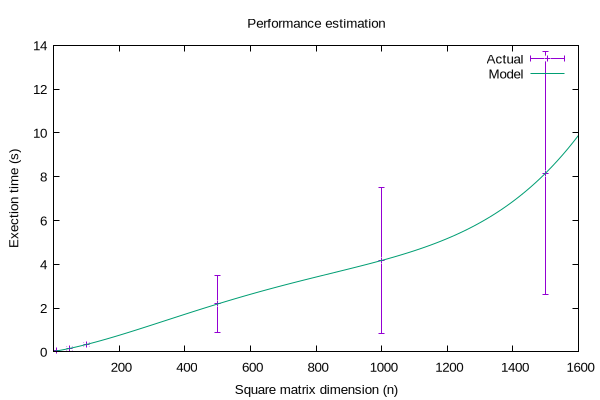
\includegraphics[width=0.9\linewidth]{func.png}
	\caption{Time needed to run func.}
	\label{fig:exectime}
\end{figure}

\begin{figure}[h!]
	\begin{minted}{shell}
gcc func.c lib.o -o func
./s2.sh -n func | sh
python3 s4.py -n func > func.dat
gnuplot -e "datafile='func.dat'; outputname='func.png'" et.gnu
	\end{minted}
	\caption{commands to reproduce the plot}\label{code:commands}
\end{figure}

\newpage

\section*{Question 4}

\subsection*{FCFS}

\begin{table}[h!]
	\centering
	\resizebox{\textwidth}{!}{
		\begin{tabular}{cc|c|c|c|c|c|c|c|c|c|c|c|c|c|c|c|c|c|c|c|c|c|c|c|c|c|c|c|c|c|c|c|c|}
			\cline{3-34}
			& & \multicolumn{32}{ c| }{Time} \\ \cline{3-34}
			& & 1 & 2 & 3 & 4 & 5 & 6 & 7 & 8 & 9 & 10 & 11 & 12 & 13 & 14 & 15 & 16 & 17 & 18 & 19 & 20 & 21 & 22 & 23 & 24 & 25 & 26 & 27 & 28 & 29 & 30 & 31 & 32 \\ \hline
			\multicolumn{1}{|c}{\multirow{10}{*}{CPU}} & \multicolumn{1}{|r|}{1} & J1 & J1 & J1 & J1 & J1 & J1 & J1 & J1 & J4 & J4 & J4 & J4 & J6 & J6 & J6 & J8 & J8 & J8 & J8 & J8 & J8 & J10 & J10 & J11 & J11 & J11 & J11 & J16 & J16 & J17 & J17 & J17 \\ \cline{2-34}
			\multicolumn{1}{|c}{} & \multicolumn{1}{|r|}{2} & J1 & J1 & J1 & J1 & J1 & J1 & J1 & J1 & J4 & J4 & J4 & J4 & J6 & J6 & J6 & J8 & J8 & J8 & J8 & J8 & J8 & J10 & J10 & J11 & J11 & J11 & J11 & J16 & J16 & J17 & J17 & J17 \\ \cline{2-34}
			\multicolumn{1}{|c}{} & \multicolumn{1}{|r|}{3} & J1 & J1 & J1 & J1 & J1 & J1 & J1 & J1 & J4 & J4 & J4 & J4 & J6 & J6 & J6 & J8 & J8 & J8 & J8 & J8 & J8 & J10 & J10 & J12 & J12 & J12 & J12 & J16 & J16 & J17 & J17 & J17 \\ \cline{2-34}
			\multicolumn{1}{|c}{} & \multicolumn{1}{|r|}{4} & J1 & J1 & J1 & J1 & J1 & J1 & J1 & J1 & J4 & J4 & J4 & J4 & J6 & J6 & J6 & J8 & J8 & J8 & J8 & J8 & J8 & J10 & J10 & J12 & J12 & J12 & J12 & J16 & J16 & J17 & J17 & J17 \\ \cline{2-34}
			\multicolumn{1}{|c}{} & \multicolumn{1}{|r|}{5} & J1 & J1 & J1 & J1 & J1 & J1 & J1 & J1 & J5 & J5 &  &  & J6 & J6 & J6 & J9 & J9 & J9 & J9 &  &  & J10 & J10 & J13 & J13 & J13 & J13 & J16 & J16 & J17 & J17 & J17 \\ \cline{2-34}
			\multicolumn{1}{|c}{} & \multicolumn{1}{|r|}{6} & J1 & J1 & J1 & J1 & J1 & J1 & J1 & J1 &  &  &  &  & J6 & J6 & J6 & J9 & J9 & J9 & J9 &  &  & J10 & J10 & J14 & J14 & J14 &  &  &  & J17 & J17 & J17 \\ \cline{2-34}
			\multicolumn{1}{|c}{} & \multicolumn{1}{|r|}{7} & J1 & J1 & J1 & J1 & J1 & J1 & J1 & J1 &  &  &  &  & J6 & J6 & J6 & J9 & J9 & J9 & J9 &  &  & J10 & J10 & J15 & J15 & J15 & J15 & J15 & J15 & J17 & J17 & J17 \\ \cline{2-34}
			\multicolumn{1}{|c}{} & \multicolumn{1}{|r|}{8} & J1 & J1 & J1 & J1 & J1 & J1 & J1 & J1 &  &  &  &  & J6 & J6 & J6 & J9 & J9 & J9 & J9 &  &  & J10 & J10 &  &  &  &  &  &  & J17 & J17 & J17 \\ \cline{2-34}
			\multicolumn{1}{|c}{} & \multicolumn{1}{|r|}{9} &  & J2 & J2 & J3 & J3 & J3 & J3 & J3 & J3 & J3 & J3 &  & J6 & J6 & J6 &  &  &  &  &  &  & J10 & J10 &  &  &  &  &  &  &  &  &  \\ \cline{2-34}
			\multicolumn{1}{|c}{} & \multicolumn{1}{|r|}{10} &  & J2 & J2 &  &  &  &  &  &  &  &  &  & J7 & J7 & J7 & J7 &  &  &  &  &  & J10 & J10 &  &  &  &  &  &  &  &  &  \\ \hline
		\end{tabular}}
	\label{tab:fcfs}
	\caption{FCFS.}
\end{table}

\subsection*{EASY-backfilling}

\begin{table}[h!]
	\resizebox{\textwidth}{!}{
		\begin{tabular}{cc|c|c|c|c|c|c|c|c|c|c|c|c|c|c|c|c|c|c|c|c|c|c|c|c|c|c|}
			\cline{3-28}
			& & \multicolumn{26}{c|}{Time} \\ \cline{3-28}
			& & 1 & 2 & 3 & 4 & 5 & 6 & 7 & 8 & 9 & 10 & 11 & 12 & 13 & 14 & 15 & 16 & 17 & 18 & 19 & 20 & 21 & 22 & 23 & 24 & 25 & 26 \\ \hline
			\multicolumn{1}{|c}{\multirow{10}{*}{CPU}} & \multicolumn{1}{|r|}{1} & J1 & J1 & J1 & J1 & J1 & J1 & J1 & J1 & J4 & J4 & J4 & J4 & J6 & J6 & J6 & J8 & J8 & J8 & J8 & J8 & J8 & J10 & J10 & J17 & J17 & J17 \\ \cline{2-28}
			\multicolumn{1}{|c}{} & \multicolumn{1}{|r|}{2} & J1 & J1 & J1 & J1 & J1 & J1 & J1 & J1 & J4 & J4 & J4 & J4 & J6 & J6 & J6 & J8 & J8 & J8 & J8 & J8 & J8 & J10 & J10 & J17 & J17 & J17 \\ \cline{2-28}
			\multicolumn{1}{|c}{} & \multicolumn{1}{|r|}{3} & J1 & J1 & J1 & J1 & J1 & J1 & J1 & J1 & J4 & J4 & J4 & J4 & J6 & J6 & J6 & J8 & J8 & J8 & J8 & J8 & J8 & J10 & J10 & J17 & J17 & J17 \\ \cline{2-28}
			\multicolumn{1}{|c}{} & \multicolumn{1}{|r|}{4} & J1 & J1 & J1 & J1 & J1 & J1 & J1 & J1 & J4 & J4 & J4 & J4 & J6 & J6 & J6 & J8 & J8 & J8 & J8 & J8 & J8 & J10 & J10 & J17 & J17 & J17 \\ \cline{2-28}
			\multicolumn{1}{|c}{} & \multicolumn{1}{|r|}{5} & J1 & J1 & J1 & J1 & J1 & J1 & J1 & J1 & J9 & J9 & J9 & J9 & J6 & J6 & J6 & J11 & J11 & J11 & J11 & J16 & J16 & J10 & J10 & J17 & J17 & J17 \\ \cline{2-28}
			\multicolumn{1}{|c}{} & \multicolumn{1}{|r|}{6} & J1 & J1 & J1 & J1 & J1 & J1 & J1 & J1 & J9 & J9 & J9 & J9 & J6 & J6 & J6 & J11 & J11 & J11 & J11 & J16 & J16 & J10 & J10 & J17 & J17 & J17 \\ \cline{2-28}
			\multicolumn{1}{|c}{} & \multicolumn{1}{|r|}{7} & J1 & J1 & J1 & J1 & J1 & J1 & J1 & J1 & J9 & J9 & J9 & J9 & J6 & J6 & J6 & J12 & J12 & J12 & J12 & J16 & J16 & J10 & J10 & J17 & J17 & J17 \\ \cline{2-28}
			\multicolumn{1}{|c}{} & \multicolumn{1}{|r|}{8} & J1 & J1 & J1 & J1 & J1 & J1 & J1 & J1 & J9 & J9 & J9 & J9 & J6 & J6 & J6 & J12 & J12 & J12 & J12 & J16 & J16 & J10 & J10 & J17 & J17 & J17 \\ \cline{2-28}
			\multicolumn{1}{|c}{} & \multicolumn{1}{|r|}{9} &  & J2 & J2 & J3 & J3 & J3 & J3 & J3 & J3 & J3 & J3 &  & J6 & J6 & J6 & J14 & J14 & J14 &  & J16 & J16 & J10 & J10 &  &  &  \\ \cline{2-28}
			\multicolumn{1}{|c}{} & \multicolumn{1}{|r|}{10} &  & J2 & J2 &  &  & J5 & J5 & J7 & J7 & J7 & J7 & J13 & J13 & J13 & J13 & J15 & J15 & J15 & J15 & J15 & J15 & J10 & J10 &  &  &  \\ \hline
		\end{tabular}}
	\label{tab:backfilling}
	\caption{EASY-backfilling - backfill does not allow delaying an existing queued job.}
\end{table}

\subsection*{Resource utilization}

\begin{table}[h!]
	\centering
	\begin{tabular}{|c|c|} 
		\hline
		Scheduling Algorithm & Resource Utilization (\%) \\ [0.5ex] 
		\hline
		FCFS & 77.5 \\
		EASY-backfilling & 95.38 \\
		\hline
	\end{tabular}
	\caption{Resource utilization (\%) for FCFS and EASY-backfilling.}
\end{table}

\end{document}
